\documentclass[12pt]{article}

\usepackage[T1]{fontenc}
\usepackage{graphicx}
\graphicspath{ {./images/} } 
\usepackage{float}
\begin{document}

(Q)
Describe: ...
\clearpage

An Introduction to \\
Distributed Systems\\
SCC 311\\
\begin{figure}[H]

\includegraphics[width=0.5\linewidth]{page1-image-1.png}
\end{figure}
\clearpage
(Q)
Describe: Overview of the Session
\clearpage
\section{Overview of the Session}
\\
■What is a distributed system?\\
■Examples of distributed systems\\
■Why distributed systems?\\
➔Historical distributed systems\\
➔Recent trends in distributed \\
systems\\
\clearpage
(Q)
Describe: What is a System?
\clearpage
\section{What is a System?}
\\
■ A collection of hardware and software.\\
■ “A computer system consists of hardware and systems \\
software that work together to run application programs.”\\
[Bryant and O'Hallaron]\\
\clearpage
(Q)
Describe: Tour of a Computer System
\clearpage
\section{Tour of a Computer System}
\\
■ Registers, L1/L2/L3 caches, RAM, local disk, remote disk\\
■ A memory hierarchy\\
■ CPU running instructions\\
Carnegie Mellon\\
76\\
Example Memory \\
Hierarchy Regs\\
L1 cache \\
(SRAM)\\
Main memory\\
(DRAM)\\
Local secondary storage\\
(local disks)\\
Larger,  \\
slower, \\
and \\
cheaper \\
(per byte)\\
storage\\
devices\\
Remote secondary storage\\
(e.g., Web servers)\\
Local disks hold files \\
retrieved from disks \\
on remote servers.\\
L2 cache \\
(SRAM)\\
L1 cache holds cache lines \\
retrieved from the L2 cache.\\
CPU registers hold words retrieved \\
from the L1 cache.\\
L2 cache holds cache lines\\
retrieved from L3 cache.\\
L0:\\
L1:\\
L2:\\
L3:\\
L4:\\
L5:\\
Smaller,\\
faster,\\
and \\
costlier\\
(per byte)\\
storage \\
devices\\
L3 cache \\
(SRAM)\\
L3 cache holds cache lines\\
retrieved from main memory.\\
L6:\\
Main memory holds disk \\
blocks retrieved from local \\
disks.\\
Carnegie Mellon\\
46\\
I/O Bus\\
Main\\
memory\\
I/O \\
bridgeBus interface\\
ALU\\
Register file\\
CPU chip\\
System bus Memory bus\\
Disk \\
controller\\
Graphics\\
adapter\\
USB\\
controller\\
Mouse Keyboard Monitor\\
Disk\\
I/O bus Expansion slots for\\
other devices such\\
as network adapters.\\
\begin{figure}[H]

\includegraphics[width=0.5\linewidth]{page4-image-1.png}
\end{figure}
\clearpage
(Q)
Describe: Tour of a Computer System
\clearpage
\section{Tour of a Computer System}
\\
■ Registers, L1/L2/L3 caches, RAM, Disk\\
■ memory hierarchy\\
■ CPU with multiple cores\\
■ Operating system\\
■ Files, threads, …\\
■ Assembly code\\
■ Compilers\\
■ Programs\\
\clearpage
(Q)
Describe: What is a Distributed System?
\clearpage
\section{What is a Distributed System?}
\\
“a collection of independent computers that appears to its \\
users as a single coherent system”\\
[Tanenbaum and van Steen]\\
“one in which hardware or software components located \\
at networked computers communicate and coordinate \\
their actions only by passing messages”\\
[Coulouris, Dollimore, Kindberg]\\
“one that stops you getting work done when a machine \\
you’ve never even heard of crashes”\\
[Lamport]\\
\clearpage
(Q)
Describe: “a system designed to support the development of 
\clearpage
\section{“a system designed to support the development of }
\\
applications and services which can exploit a physical \\
architecture consisting of multiple autonomous \\
processing elements that do not share primary memory \\
but cooperate by sending asynchronous messages over \\
a communications network”\\
[Blair and Stefani, 1998]\\
What is a Distributed System?\\
\clearpage
(Q)
Describe: In its broadest definition, a distributed system is one that 
\clearpage
\section{In its broadest definition, a distributed system is one that }
\\
comprises more than one computer with the goal of \\
reaching a level of performance and/or providing a \\
service that is quite difficult or infeasible to do on a single \\
computer.\\
What is a Distributed System?\\
\begin{figure}[H]

\includegraphics[width=0.5\linewidth]{page8-image-1.png}
\end{figure}
\clearpage
(Q)
Describe: Examples of Distributed Systems
\clearpage
\section{Examples of Distributed Systems}
\\
■ Financial trading\\
➔ Support execution of trading transactions\\
➔ Dissemination and processing of events\\
■ Web search\\
➔ The web consists of over 6 billion web pages across 8.2 \\
million servers with an average lifetime of about 2 months.\\
➔ Modern web engines serve over 3.5 billion searches per day\\
 \textgreater  Major distributed systems challenges\\
■ Massively multiplayer online games\\
➔ Online games (e.g. Fortnite, Among Us) support large \\
numbers of users viewing and changing a common world\\
➔ Need for very low latency coordination to support gameplay\\
\begin{figure}[H]

\includegraphics[width=0.5\linewidth]{page9-image-1.png}
\end{figure}
\clearpage
(Q)
Describe: Why Distributed Systems?
\clearpage
\section{Why Distributed Systems?}
\\
■ Because the world is distributed\\
➔ You want to book a hotel in Sydney, but you are in Lancaster\\
➔ You want to be able to retrieve money from any ATM in the world, \\
but your bank is in London\\
➔ An airplane has 1 cockpit, 2 wings, 4 engines, 10k sensors, etc.\\
0 Similarly railway networks, and other distributed transport systems\\
■ Because problems rarely hit two different places at the same \\
time\\
➔ As a company having only one database server is a bad idea\\
➔ Having two in the same room is better, but still risky\\
■ Because joining forces increases performance, availability, etc.\\
➔ High Performance Computing, replicated web servers, etc.\\
\clearpage
(Q)
Describe: Why Distributed Systems?
\clearpage
\section{Why Distributed Systems?}
\\
\begin{figure}[H]

\includegraphics[width=0.5\linewidth]{page11-image-1.png}
\end{figure}
\clearpage
(Q)
Describe: Is this important?
\clearpage
\section{Is this important?}
\\
\begin{figure}[H]

\includegraphics[width=0.5\linewidth]{page12-image-1.png}
\end{figure}
\begin{figure}[H]

\includegraphics[width=0.5\linewidth]{page12-image-2.png}
\end{figure}
\begin{figure}[H]
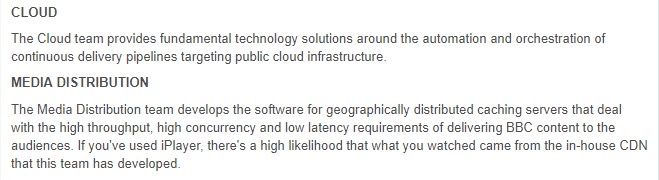
\includegraphics[width=0.5\linewidth]{page12-image-3.png}
\end{figure}
\begin{figure}[H]
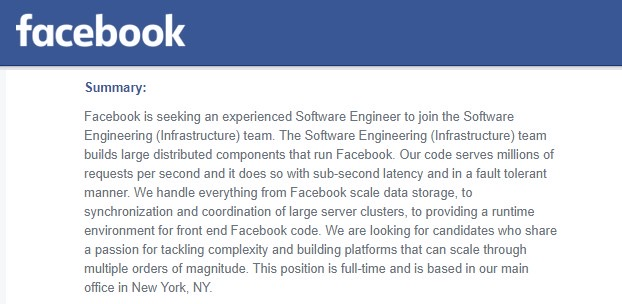
\includegraphics[width=0.5\linewidth]{page12-image-4.png}
\end{figure}
\begin{figure}[H]

\includegraphics[width=0.5\linewidth]{page12-image-5.png}
\end{figure}
\begin{figure}[H]

\includegraphics[width=0.5\linewidth]{page12-image-6.png}
\end{figure}
\begin{figure}[H]

\includegraphics[width=0.5\linewidth]{page12-image-7.png}
\end{figure}
\clearpage
(Q)
Describe: A Short History of DSs
\clearpage
\section{A Short History of DSs}
\\
■ Distributed Computer Systems are largely concerned with:\\
➔ Data processing/ management/ presentation (“computing” side)\\
➔ Communication/ coordination (“distributed side”)\\
■ Those concerns existed well before computers were invented\\
➔ Ancient civilisations needed efficient communication:\\
0 cf. the Postal Service of the Persian Empire (6th century BC), \\
the Roman roads (many still visible today), etc.\\
0 assuming a good infrastructure (roads, horses, staging posts)\\
0 max message speed: \~ 200 miles/day in the Persian system\\
➔ Delays impose distributed organisations\\
0 Persian and Roman empires extended over 1000s of miles\\
➔ Trust / secrecy / reliability issues\\
0 Am I sure Governor X is doing what he says he is?\\
■ This all has not really changed! \\
Things have only sped up.\\
\begin{figure}[H]

\includegraphics[width=0.5\linewidth]{page13-image-1.png}
\end{figure}
\begin{figure}[H]

\includegraphics[width=0.5\linewidth]{page13-image-2.png}
\end{figure}
\clearpage
(Q)
Describe: A Short History of DSs
\clearpage
\section{A Short History of DSs}
\\
■ Computers are far more recent\\
➔ The first “modern” computers appeared just after WWII\\
➔ They were slow, bulky, and incredibly expensive\\
0 The ENIAC (1945), used by the US army: 30 tons, 170 m2 footprint,\\
180 kilowatts, 18,000 vacuum tubes, and 5,000 additions/second (5KHz),\\
0 Price: \$500,000 (in US\$ of the time, would be  \textgreater  \$5,000,000 today)\\
■ And distributed computing is even more recent\\
➔ For a long time, only very few computers were around anyway\\
➔ No practical technology to connect them\\
➔ This all changed in the 80’s:\\
0 The rise of the micro-computers (PC, Mac, etc.)\\
0 The launch of the “Internet” (1982, TCP/IP), after 10 years of development\\
1940s 50s 60s 70s 80s 90s 00s 10s 20s\\
Fir\\
st\\
co\\
m\\
pu\\
ter\\
M\\
ain\\
fra\\
m\\
es\\
Mi\\
cro\\
-co\\
m\\
pu\\
ter\\
s\\
Th\\
e W\\
W\\
W\\
Gr\\
id\\
co\\
m\\
pu\\
tin\\
g\\
P2\\
P\\
co\\
m\\
pu\\
tin\\
g\\
Int\\
er\\
ne\\
t o\\
f T\\
hin\\
gs\\
Cl\\
ou\\
d c\\
om\\
pu\\
tin\\
g\\
Fo\\
g c\\
om\\
pu\\
tin\\
g\\
M\\
ini\\
-co\\
m\\
pu\\
ter\\
s\\
\begin{figure}[H]

\includegraphics[width=0.5\linewidth]{page14-image-1.png}
\end{figure}
\begin{figure}[H]

\includegraphics[width=0.5\linewidth]{page14-image-2.png}
\end{figure}
\clearpage
(Q)
Describe: Recent Trends
\clearpage
\section{Recent Trends}
\\
■ Pervasive networking and the modern Internet\\
➔ Highly heterogeneous networking technologies\\
➔ Fusion of services (telephony, broadcasting…)\\
■ Mobile and ubiquitous computing\\
➔ Personal devices and embedded systems\\
■ Distributed multimedia systems\\
➔ IPTV and Voice over IP services\\
■ Distributed computing as a utility\\
➔ Grid, Cloud, and Fog computing\\
■ The pace of change is accelerating\\
\begin{figure}[H]

\includegraphics[width=0.5\linewidth]{page15-image-1.png}
\end{figure}
\begin{figure}[H]

\includegraphics[width=0.5\linewidth]{page15-image-2.png}
\end{figure}
\begin{figure}[H]
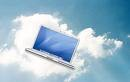
\includegraphics[width=0.5\linewidth]{page15-image-3.png}
\end{figure}
\begin{figure}[H]
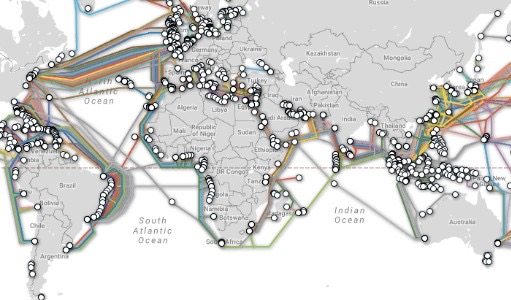
\includegraphics[width=0.5\linewidth]{page15-image-4.png}
\end{figure}
\clearpage
(Q)
Describe: Interactions
\clearpage
\section{Interactions}
\\
■ What sort of interactions do we expect?\\
■ Web\\
➔ Client: “I want this thing”\\
➔ Server: “Here’s the thing”\\
■ eBay\\
➔ Alice: “I bid £10”\\
➔ Bob: “I bid £12”\\
➔ eBay: “Alice wins. Bob was late”\\
■ More on design patterns later (week 4).\\
\begin{figure}[H]

\includegraphics[width=0.5\linewidth]{page16-image-1.png}
\end{figure}
\begin{figure}[H]

\includegraphics[width=0.5\linewidth]{page16-image-2.png}
\end{figure}
\clearpage
(Q)
Describe: Is this easy?
\clearpage
\section{Is this easy?}
\\
\begin{figure}[H]

\includegraphics[width=0.5\linewidth]{page17-image-1.png}
\end{figure}
\clearpage
(Q)
Describe: But why is this so hard?
\clearpage
\section{But why is this so hard?}
\\
■ A bank asks you to program their new ATM software\\
➔ Central bank computer (server) stores account information\\
➔ Remote ATMs authenticate customers and deliver money\\
■ A first version of the program\\
➔ ATM: (ignoring authentication and security issues)\\
1. Ask customer how much money s/he wants\\
2. Send message with  \textless customer ID, withdraw, amount \textgreater  to bank server\\
3. Wait for bank server answer:  \textless OK \textgreater  or  \textless refused \textgreater \\
4. If  \textless OK \textgreater  give money to customer, else display error message\\
➔ Central Server:\\
1. Wait for messages from ATM:  \textless customer ID, withdraw, amount \textgreater \\
2. If enough money withdraw money, send  \textless OK \textgreater , else send  \textless refused \textgreater \\
\clearpage
(Q)
Describe: ATM Bank Server
\clearpage
\section{ATM Bank Server}
\\
John: £500\\
■ But ...\\
➔ What if the bank server crashes just after 2 and before 3?\\
➔ What if the  \textless OK \textgreater  message gets lost? Takes too long to arrive?\\
➔ What if the ATM crashes after 1, but before 4?\\
■ More on challenges in coming lectures.\\
 \textless  John, withdraw, £200  \textgreater \\
1\\
John: £300\\
-£200 2\\
 \textless OK \textgreater \\
3\\
4\\
But why is this so hard?\\
\begin{figure}[H]

\includegraphics[width=0.5\linewidth]{page19-image-1.png}
\end{figure}
\begin{figure}[H]

\includegraphics[width=0.5\linewidth]{page19-image-2.png}
\end{figure}
\begin{figure}[H]

\includegraphics[width=0.5\linewidth]{page19-image-3.png}
\end{figure}
\begin{figure}[H]
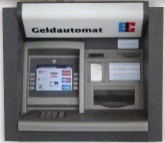
\includegraphics[width=0.5\linewidth]{page19-image-4.png}
\end{figure}
\clearpage
(Q)
Describe: Is this easy?
\clearpage
\section{Is this easy?}
\\
\begin{figure}[H]

\includegraphics[width=0.5\linewidth]{page20-image-1.png}
\end{figure}
\clearpage
(Q)
Describe: Expected Learning Outcomes
\clearpage
\section{Expected Learning Outcomes}
\\
At the end of this session, you should be able to:\\
■ Define distributed computer systems\\
■ Explain why distribution is needed\\
■ Know a few everyday examples of distributed systems\\
■ Understand how they evolved into their current form\\
\clearpage
(Q)
Describe: Additional Reading
\clearpage
\section{Additional Reading}
\\
■ Required: CDKB, chapter 1 sections 1.1 -- 1.4\\
➔ also chapter 3 for revision\\
■ TvS, chapter 1\\
■ Computer Systems: A Programmer's Perspective, by Bryant \\
and O'Hallaron, chapter 1\\
■ Mark Cavage, “There's Just No Getting around It: You're \\
Building a Distributed System”, ACM Queue, Vol. 11 No. 4, \\
April 2013. http://queue.acm.org/detail.cfm?id=2482856\\
\clearpage
(Q)
Describe: ...
\clearpage
\clearpage
(Q)
Describe: ...
\clearpage
\\
\end{document}